\documentclass[12pt, dvipsnames, svgnames, x11names, oneside]{book}

% Packages --------------------------------------------------
\usepackage{dirtytalk}
\usepackage{quotchap}
\usepackage{epigraph} 
\usepackage{paralist}
\usepackage{pdfpages}
%------------------------------------------------------------

% URLs and hyperlinks ---------------------------------------
\usepackage{hyperref}
\hypersetup{
	colorlinks=true,
	linkcolor=Navy,
	filecolor=magenta,      
	urlcolor=Navy,
	pdftitle=Plann,
}
\usepackage{xurl}
%------------------------------------------------------------

% colorbox --------------------------------------------------
\usepackage{tcolorbox}

\newcommand{\colourbox}[2]{
    \tcbox[on line, 
	 		boxsep=4pt, 
	 		left=0pt,
	 		right=0pt,
	 		top=0pt,
	 		bottom=-1pt,
	 		colframe=white,
	 		colback={#1},  
	 		size=small
	]{#2}
}
%------------------------------------------------------------

% footnotes in headings -------------------------------------
\usepackage[stable]{footmisc}
%------------------------------------------------------------

% Tags ------------------------------------------------------
\newcommand{\mustread}{{\small\colourbox{red!85!}{\texttt{must-be-read}}}}
\newcommand{\betteread}{{\small\colourbox{Dandelion}{\texttt{better-to-read}}}}
\newcommand{\laterread}{{\small\colourbox{DarkGray!70!}{\texttt{later-to-read}}}}
\newcommand{\bookread}{{\small\normalfont\colourbox{Gold}{\texttt{read}}}}
\newcommand{\printed}{{\small\normalfont\colourbox{DeepSkyBlue}{\texttt{printed}}}}

\newcommand{\nearonethpages}{{\small\colourbox{DarkOrchid3!75!}{\texttt{near-one-thousand-pages}}}}
\newcommand{\nearsevenhpages}{{\small\colourbox{DeepPink!85!}{\texttt{near-seven-hundred-pages}}}}
\newcommand{\nearfivehpages}{{\small\colourbox{DeepPink!55!}{\texttt{near-five-hundred-pages}}}}
\newcommand{\neartwohpages}{{\small\colourbox{Violet!60!}{\texttt{near-two-hundred-pages}}}}

\newcommand{\pricenearfive}[1]{{\small\colourbox{Green3}{\texttt{{#1} T}}}}
\newcommand{\pricenearfour}[1]{{\small\colourbox{Green3!65!}{\texttt{{#1} T}}}}
\newcommand{\pricenearthree}[1]{{\small\colourbox{Green3!55!}{\texttt{{#1} T}}}}
\newcommand{\priceneartwo}[1]{{\small\colourbox{Green3!35!}{\texttt{{#1} T}}}}
\newcommand{\pricenearone}[1]{{\small\colourbox{Green3!15!}{\texttt{{#1} T}}}}

\newcommand{\always}{{\small\normalfont\colourbox{red}{\texttt{always}}}}
\newcommand{\weekend}{{\small\normalfont\colourbox{DarkOrchid3!75!}{\texttt{weekends}}}}
\newcommand{\timetotime}{{\small\normalfont\colourbox{Dandelion}{\texttt{time-to-time}}}}
\newcommand{\normal}{{\small\normalfont\colourbox{DarkGray!70!}{\texttt{activity}}}}
\newcommand{\rest}{{\small\normalfont\colourbox{DeepPink!85!}{\texttt{rest}}}}
\newcommand{\para}[1]{\noindent{#1}\newline}

\newcommand{\hard}{{\small\normalfont\colourbox{DarkMagenta!70!}{\texttt{Hard}}}}
\newcommand{\easy}{{\small\normalfont\colourbox{Yellow}{\texttt{Easy}}}}

\newcommand{\longvideo}{{\small\normalfont\colourbox{CadetBlue2}{\texttt{Long}}}}
\newcommand{\shortvideo}{{\small\normalfont\colourbox{LightBlue1}{\texttt{Short}}}}

\newcommand{\many}{{\small\normalfont\colourbox{DeepPink2}{\texttt{Many}}}}
%------------------------------------------------------------

% Including pictures ----------------------------------------
\usepackage{tikz}
\usepackage{graphicx}
\newcommand{\bookcover}[1]{
	\begin{center}
		\includegraphics[width=8cm, height=10cm]{{#1}}
	\end{center}
}

\newcommand{\roundpic}[4][]{
	\tikz\node [circle, minimum width = #2,
	path picture = {
		\node [#1] at (path picture bounding box.center) {
			\includegraphics[width=#3]{#4}};
	}] {};}
%------------------------------------------------------------

% Title, author and date ------------------------------------
\title{\roundpic[xshift=-3mm,yshift=-5mm]{5.8cm}{9cm}{./images/lamp}\vspace{3mm}
	
	My Learning Plan
}
\author{Mahdi Haghverdi} 
%------------------------------------------------------------

% environments ----------------------------------------------
\newenvironment{sansserif}{\sffamily}{\normalfont}
%------------------------------------------------------------

\begin{document}
	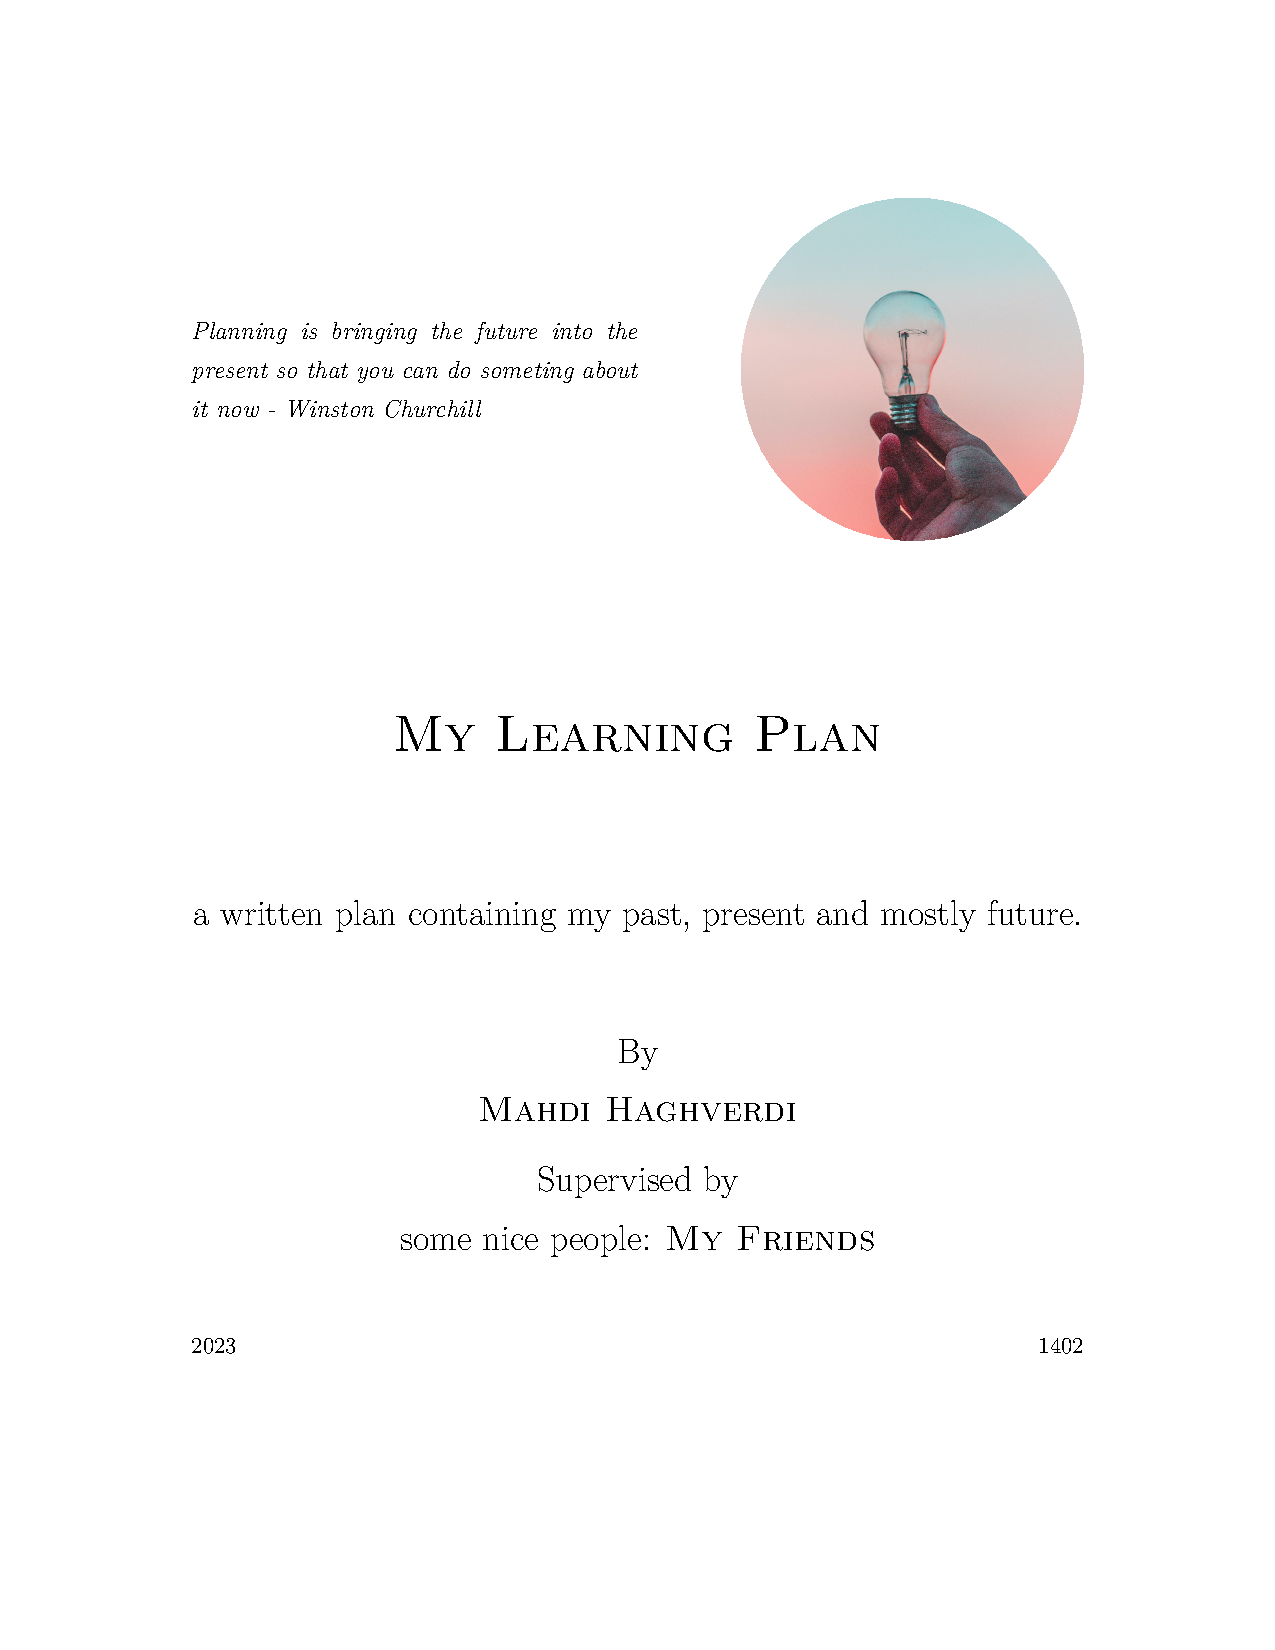
\includepdf{butterflytitle}
	\frontmatter
	\tableofcontents
	\clearpage
	\chapter{\textsf{Preface}}	
		\para{After going up and down in my life, I finally found the way to study and learn well. This document has everything I want to do and resource I want to check. This plan will be started from the summer of 1402 (2023.)}
			
		\para{After spending one whole semester in the university\footnote{the 3rd semester}, it is got clear to me, that \underline{meanwhile} studying, learning \textbf{new}  things, is hard! It's possible but it's hard. So summers are the times which I have to value a lot and to make the most outta 'em.}
		
		\para{At the time of writing this, there are 5 days remaining of the year, a long and hard year both for Iran, my love, and myself. I learned and grew a lot during this year. I spend a whole semester in university, experienced a really \textit{Randomly-Generated-but-Related} journey. Studied a lot, learned how to study well and meet many new and nice people.}
		
		
		\para{But after all, I have to create a path to my actual career! This is the most important thing which I have to take care of. After working, searching and talking to many people, I've finally made my decision and chosen: \textit{Data Science}. I really like this field, it's very amazing but hard to learn :) Beside this, I wanna learn backend engineering as well, 'cause it is much faster (faster to get result, lol) and has a slightly smaller learning curve.}
		
		\para{This plan will be started from the summer of 1402 (2023), but I will be working and adding things to this document from time to time; there may be some new chapters or reorganization of the chapter but not now \textsf{:D}}
		
		\para{This will be a hot summer. It gets hot because of so many hours I want to study, both with video courses and with reading books. To learn data science I asked someone in our university who already is a data scientist, and he introduced me to the deep learning course of \textit{Jeremy Howard}. This course is freely available on YouTube. Also this course needs a book nearby (written by Jeremy Howard) called \textit{Deep Learning for Coders With Fastai and PyTorch}.}
		
		\para{Besides learning data science, learning new things and refreshing my Python skills is something that I would never miss and enjoy a lot. The focus of this summer will be on the CPython implementation itself, so I've chosen some nice books on this field. I have gathered some more general books on Python too, but they would have a lesser priority.}
		
		\para{Watching video courses and reading books are the main activities of the summer, but without spending or more precisely, \textit{acquiring} time to rest, nobody can learn anything; listening to music and podcast and watching movies are the main non-active and biking is the main physical activity of my summer.}


	\mainmatter		
	
	\begin{savequote}[80mm]
		Some knowledge needs to be learned by video courses, and then be completed by reading books and researching in a long journey.
		\qauthor{Me}			
	\end{savequote}
	\chapter{Courses}
		\begin{sansserif}
			\para{Well, the major part of the summer is the courses, in this chapter I will introduce the courses I want to watch and some useful information about them.}
			
			\noindent Eash course is tagged with these:
			\begin{itemize}
				\item Learning curse
				\begin{itemize}
					\item \hard
					\item \easy
				\end{itemize}
				\item Video duration
				\begin{itemize}
					\item \longvideo
					\item \shortvideo
				\end{itemize}
				\item Video Count: \many
			\end{itemize}
		\end{sansserif}
		
		\clearpage		
		\section{Deep learning}
		\epigraph{
			\begin{sansserif}
				The career I chose, \say{The sexiest job of the 21st century,} \say{The best job in America,} \say{One of the newest and coolest jobs in IT world}
			\end{sansserif}
		}
		
		\begin{inparadesc}
			\item \hard
			\item \longvideo
		\end{inparadesc}
		\vspace{3mm}
		
		\para{Well as the quote says, this is exciting, BUT it really needs knowledge and effort to gain, the starting point is here: this nice deep learning course at \url{https://course.fast.ai/}.}
		
		\para{\textbf{Practical Deep Learning}}
		\para{\textit{A free course designed for people with some coding experience, who want to learn how to apply deep learning and machine learning to practical problems.}}
		
		\para{\textit{This free course is designed for people (and bunnies!) with some coding experience who want to learn how to apply deep learning and machine learning to practical problems.}}
		
		\para{Each lesson of the course has a video and a dedicated page of the website, like \href{https://course.fast.ai/Lessons/lesson1.html}{Lesson 1}. }
		
		\noindent Notes:
		\begin{itemize}
			\item Each video is pretty long, on average they last one hour and 30 minutes! The longer the video, the more knowledge they contain AND the more attention they need AND the more practice as well.
			
			\item Each lesson has a \textit{How to complete lesson N} section (like \href{https://course.fast.ai/Lessons/lesson1.html#how-to-complete-lesson-1}{here},) in which says: \textit{As well as watching the video and working through the notebooks, you should also read the relevent chapter(s) of the fast.ai book, Practical Deep Learning for Coders. Each lesson will tell you what chapter you need to read, just below the video}
		\end{itemize}
		
		After all, \textsf{the dedicated time and effort must be huge.}
		
		\clearpage
		\section{FastAPI}
		\epigraph{
			\begin{sansserif}
				\say{FastAPI framework, high performance, easy to learn, fast to code, ready for production}
			\end{sansserif}	
		}{\href{https://fastapi.tiangolo.com}{fastapi.tiangolo.com}}
		
		\begin{inparadesc}
			\item \easy
			\item \shortvideo
			\item \many
		\end{inparadesc}
		\vspace{3mm}
		
		\para{We all know FastAPI and there is no need for more introduction.
			The course I wanna watch is \url{https://youtu.be/0sOvCWFmrtA}}
		
		\noindent The course is a 19-hour long video which is downloaded and cut already. The important things are:
		\begin{itemize}
			\item The course is created one year ago and it is slightly outdated, so the \href{https://fastapi.tiangolo.com}{documentation} must be read along the course.
			
			\item Course will just show you how to use FastAPI and the real learning happens when doing projects.
			
			\item It's good to define nice projects whenever I came to an idea
			e.g. \textit{The API to send pictures of \url{https://unsplash.com} to my friends} :)
		\end{itemize}
		
		
		\clearpage
		\section{From Deep Learning Foundations to Stable Diffusion}
		
		\para{Three years ago we pioneered Deep Learning from the Foundations, an in depth course that started right from the foundations—implementing and GPU-optimising matrix multiplications and initialisations—and covered from scratch implementations of all the key applications of the fastai library.}
		
		\para{This year, we’re going \say{from the foundations} again, but this time we’re going further. \textbf{Much} further! This time, we’re going all the way through to implementing the astounding Stable Diffusion\footnote{\url{https://stability.ai/blog/stable-diffusion-public-release}} algorithm. That’s the killer app\footnote{\url{https://www.pcworld.com/article/916785/creating-ai-art-local-pc-stable-diffusion.html}} that made the internet freak out\footnote{\url{https://devops.com/stable-diffusion-public-richixbw/}}, and caused the media to say\footnote{\url{https://arstechnica.com/information-technology/2022/09/with-stable-diffusion-you-may-never-believe-what-you-see-online-again/}} \say{you may never believe what you see online again}.}
		
		\para{Stable diffusion, and diffusion methods in general, are a great learning goal for many reasons. For one thing, of course, you can create amazing stuff with these algorithms! To really take the technique to the next level, and create things that no-one has seen before, you need to really deeply understand what’s happening under the hood. With this understanding, you can craft your own loss functions, initialization methods, multi-model mixups, and more, to create totally new applications that have never been seen before.}
		
		\para{Just as important: it’s a great learning goal because nearly every key technique in modern deep learning comes together in these methods. Contrastive learning, transformer models, auto-encoders, CLIP embeddings, latent variables, u-nets, resnets, and much more are involved in creating a single image.}
		
		\para{This is all cutting-edge stuff, so to ensure we bring the latest techniques to you, we’re teaming up with the folks that brought stable diffusion to the world: \url{stability.ai}. stability.ai are, in many ways, kindred spirits to fast.ai. They are, like us, a self-funded research lab. And like us, their focus is smashing down any gates that make cutting edge AI less accessible. So it makes sense for us to team up on this audacious goal of teaching stable diffusion from the foundations.}
		
		\para{The course will be available for free online from early 2023. But if you want to join the course right as it’s made, along with hundreds of the world’s leading deep learning practitioners, then you can register to join the virtual live course\footnote{\url{https://itee.uq.edu.au/event/2022/practical-deep-learning-coders-uq-fastai-part-2}} through our official academic partner, the University of Queensland (UQ). UQ will have registrations open in the next few days, so keep an eye on the link above.}
		
		\para{During the live course, we’ll be learning to read and implement the latest papers, with lots of opportunity to practice and get feedback. Many past participants in fast.ai’s live courses have described it as a “life changing” experience… and it’s our sincere hope that this course will be our best ever.}
		
		\para{To get the most out of this course, you should be a reasonably confident deep learning practitioner. If you’ve finished fast.ai’s Practical Deep Learning course\footnote{text\url{https://course.fast.ai/}} then you’ll be ready! If you haven’t done that course, but are comfortable with building an SGD training loop from scratch in Python, being competitive in Kaggle competitions, using modern NLP and computer vision algorithms for practical problems, and working with PyTorch and fastai, then you will be ready to start the course. (If you’re not sure, then I strongly recommend getting starting with Practical Deep Learning now—if you push, you’ll be done before the new course starts!)}
		
		\para{If you’re an alumnus of Deep Learning for Coders, you’ll know that course sets you up to be an effective deep learning practitioner. This new course will take you to the next level, creating novel applications that bring multiple techniques together, and understanding and implementing research papers. Alumni of previous versions of fast.ai’s “part 2” courses have even gone on to publish deep learning papers in top conferences and journals, and have joined highly regarded research labs and startups.}
	
	
	\begin{savequote}[80mm]
		I find television very educating. Every time somebody turns on the set, I go into the other room and read a book.
		\qauthor{Groucho Marx}
		
		There is more treasure in books than in all the pirate’s loot on Treasure Island.
		\qauthor{Walt Disney}	
	\end{savequote}
	\chapter{Books}
		\para{\textsf{You may argue me about what I want to say, however I found it true: \say{If you want to learn \textit{something}, the real source is the books about it.} This is absolutely true. No video course and no article and nothing else may contain the most valuable information about something. All the video courses and simple article ARE come from the books.}}
		
		\para{\textsf{In this chapter I may introduce many invaluable books (most technical books but it may contain other books as well.)}}
		
		\noindent\textsf{Each section of this chapter has the name of the book which is a link to the post of that book in the store: \url{Skybooks.ir}, where I buy the books from. Then there maybe some tags under the name of the books, the whole tags are categorized in three categories:}
		\sffamily
		\begin{enumerate}
			\item Reading priority
				\begin{itemize}
					\item \mustread
					\item \betteread
					\item \laterread
				\end{itemize}
			\item Buying considerations:
				\begin{enumerate}
					\item Number of pages
						\begin{itemize}
							\item \nearonethpages
							\item \nearsevenhpages
							\item \nearfivehpages
							\item \neartwohpages
						\end{itemize}
					\item Price:
						\begin{itemize}
							\item \pricenearfive{number}
							\item \pricenearfour{number}
					        \item \pricenearthree{number}
							\item \priceneartwo{number}
							\item \pricenearone{number}
						\end{itemize}
				\end{enumerate}
			\item Book read \bookread
		\end{enumerate}
		\normalfont
	    \clearpage
	    
		\section{\href{https://skybooks.ir/products/Deep-Learning-for-Coders-with-fastai-and-PyTorch}{Deep Learning for Coders With Fastai and PyTorch}}
			
			\begin{inparadesc}
				\item \mustread
				\item \nearsevenhpages
				\item \pricenearfour{297}
			\end{inparadesc}
			\vspace{3mm}
			
			\bookcover{deeplearning}
						
			\para{Deep learning is often viewed as the exclusive domain of math PhDs and big tech companies. But as this hands-on guide demonstrates, programmers comfortable with Python can achieve impressive results in deep learning with little math background, small amounts of data, and minimal code. How? With fastai, the first library to provide a consistent interface to the most frequently used deep learning applications show you how to train a model on a wide range of tasks using fastai and PyTorch.} 
			
			\para{You'll also dive progressively further into deep learning theory to gain a complete understanding of the algorithms behind the scenes. Train models in computer vision, natural language processing, tabular data, and collaborative filtering Learn the latest deep learning techniques that matter most in practice Improve accuracy, speed, and reliability by understanding how deep learning models work Discover how to turn your models into web applications Implement deep learning algorithms from scratch Consider the ethical implications of your work.}
			
			\para{\sffamily As a 622-page and comprehensive book, it needs attention and time. The book may get printed, just to be read easily.}
		
		\clearpage
		\section{\href{https://skybooks.ir/products/Fluent-Python}{Fluent Python}}
			\begin{inparadesc}
				\item \laterread
				\item \nearonethpages
				\item \pricenearfive{505}
			\end{inparadesc}
			\vspace{3mm}
			
			\bookcover{fluent}
			
			\para{Python’s simplicity lets you become productive quickly, but often this means you aren’t using everything it has to offer. With the updated edition of this hands-on guide, you’ll learn how to write effective, modern Python 3 code by leveraging its best ideas. Don’t waste time bending Python to fit patterns you learned in other languages. Discover and apply idiomatic Python 3 features beyond your past experience. Author Luciano Ramalho guides you through Python’s core language features and libraries and teaches you how to make your code shorter, faster, and more readable.} 
			
			\noindent Featuring major updates throughout the book, Fluent Python, second edition, covers:
			\begin{enumerate}
				\item Special methods: The key to the consistent behavior of Python objects
				\item Data structures: Sequences, dicts, sets, Unicode, and data classes
				\item Functions as objects: First-class functions, related design patterns, and type hints in function declarations
				\item Object-oriented idioms: Composition, inheritance, mixins, interfaces, operator overloading, static typing and protocols
				\item Control flow: Context managers, generators, coroutines, async/await, and thread/process pools
				\item Metaprogramming: Properties, attribute descriptors, class decorators, and new class metaprogramming hooks that are simpler than metaclasses
			\end{enumerate}
		
		\clearpage
		\section{\href{https://skybooks.ir/products/Build-a-Career-in-Data-Science}{Build a Career in Data Science}}
			\begin{inparadesc}
				\item \laterread
				\item \nearfivehpages
				\item \pricenearthree{194}
			\end{inparadesc}
			\vspace{3mm}
			
			\bookcover{career}
			
			\para{What are the keys to a data scientist's long-term success? Blending your technical know-how with the right "soft skills" turns out to be a central ingredient of a rewarding career.} 
			
			\para{Build a Career in Data Science is your guide to landing your first data science job and developing into a valued senior employee. By following clear and simple instructions, you'll learn to craft an amazing resumé and ace your interviews.} 
			
			\para{In this demanding, rapidly changing field, it can be challenging to keep projects on track, adapt to company needs, and manage tricky stakeholders. You'll love the insights on how to handle expectations, deal with failures, and plan your career path in the stories from seasoned data scientists included in the book.} 
			
			\noindent What's Inside:
			\begin{inparaitem}
				\item Creating a portfolio of data science projects
				\item Assessing and negotiating an offer
				\item Leaving gracefully and moving up the ladder
				\item Interviews with professional data scientistsFor readers who want to begin or advance a data science career.
			\end{inparaitem} \newline
			
			\para{Emily Robinson is a data scientist at Warby Parker.Jacqueline Nolis is a data science consultant and mentor.}
		
		\clearpage
		\section{\href{https://skybooks.ir/products/Inside-The-Python-Virtual-Machine}{Inside the Python Virtual Machine}}\label{ipvm}
			\begin{inparadesc}
				\item \betteread
				\item \neartwohpages
				\item \pricenearone{108}
			\end{inparadesc}
			\vspace{3mm}
	
			\bookcover{insidepyvenv}
						
			\para{Inside the Python Virtual Machine provides a guided tour under the covers of the Python interpreter for the curious pythonista. It attempts to show the user what happens from the moment the user executes a piece of Python code to the point when the interpreter returns the result of executing the piece of code.}
			
			\para{This book will provide the readers with an understanding of the various processes that go into compiling and executing a python program removing most of the mystery surrounding how the python interpreter executes source code.} 
			
			\para{The books starts out with a description of the compilation phase with emphasis on the less generic parts of the compilation phase. It then proceeds to discuss python objects and their implementation in CPython.  This is followed by a discussion of various objects types that are central to the interpreter such as frame objects and code objects. The process of evaluating code objects by the interpreter loop is also discussed as well as how to extend the Python programming language with your own constructs.}
			
		\clearpage
		\section{\href{https://skybooks.ir/products/CPython-Internals}{CPython Internals}}		
			\begin{inparadesc}
				\item \betteread
				\item \nearfivehpages
				\item \pricenearthree{209}
			\end{inparadesc}
			\vspace{3mm}
			
			\bookcover{internals}
			
			\para{CPython Internals: Your Guide to the Python 3 Interpreter.}
			
			\para{Are there certain parts of Python that just seem like magic? Once you see how Python works at the interpreter level, you’ll be able to optimize your applications and fully leverage the power of Python.}
			
			\para{In CPython Internals, you’ll unlock the inner workings of the Python language, learn how to compile the Python interpreter from source code, and cover what you’ll need to know to confidently start contributing to CPython yourself!}	
	
	\begin{savequote}[80mm]
		Replacing just a few key negative habits with a few positive habits can easily be the difference between being mostly unhappy and being happy almost all of the time.
		\qauthor{Tynan, Superhuman by Habit}			
	\end{savequote}
	\chapter{Habits}
	\begin{sansserif}
		\para{To continue to live and rest I found some ways to spend my leisure time, just like the books they've got small tags to make them more clear.}
		
		\noindent The tags:
		\begin{enumerate}
			\item \always which says this item has no specific time.
			\item \weekend the weekends are good for this item
			\item \timetotime you can do it whenever you want to
			\item \normal needs body activity
			\item \rest	is done to rest and NOT to think about anything else
		\end{enumerate}
	\end{sansserif}

		\section{Podcast}
			\epigraph{
				\begin{sansserif}
					 \say{Listening to podcast, reading a book, listening to an audiobook and watching films isn’t waste of time. It’s how somebody becomes wise!}
				\end{sansserif}	
			}{Deyth Banger}
		
			\begin{inparadesc}
				\item \timetotime
				\item \normal
			\end{inparadesc}
			\vspace{2mm}
			
			\para{Talk Python to Me is a weekly podcast hosted by developer and entrepreneur Michael Kennedy. We dive deep into the popular packages and software developers, data scientists, and incredible hobbyists doing amazing things with Python. If you're new to Python, you'll quickly learn the ins and outs of the community by hearing from the leaders. And if you've been Pythoning for years, you'll learn about your favorite packages and the hot new ones coming out of open source.}
						
			\para{Listening to old and new Python podcasts, specially from \textit{Talk Python to Me} channel helps a lot, It provides many information, introduces mane new technologies and brings many good people to the show.}
			
		\section{Music}
			\epigraph{
				\begin{sansserif}
					\say{Music doesn't lie. If there is something to be changed in this world, then it can only happen through music.}
				\end{sansserif}
		    }{Jimi Hendrix}

			\begin{inparadesc}
				\item \always
			\end{inparadesc}
			\vspace{2mm}
		
			\para{As always: \textit{I live because of my musics} :)}
			
		\section{Films}
			\epigraph{
				\begin{sansserif}
					\say{Movies are like an expensive form of therapy for me.
				\end{sansserif}
			}}{Tim Burton}
		
			\begin{inparadesc}
				\item \weekend
				\item \rest
			\end{inparadesc}
			\vspace{2mm}
			
			\para{Watching new films and series, enjoys a LOT. The dedicated series which I want to watch is \textit{The Mentalist}. A TV show which remembers me of Sherlock!}
			
			\para{Also I will download the films which I haven't watch in 1080p quality and enjoy the leisure :)}
			
		\section{Biking}
			\epigraph{
				\begin{sansserif}
					\say{Life is like riding a bicycle. To keep your balance you must keep moving}
				\end{sansserif}	
			}{Albert Einstein}
			
			\begin{inparadesc}
				\item \timetotime
				\item \normal
			\end{inparadesc}
			\vspace{2mm}

			\para{Physical activity to become fresh again, and to empty the mind outta the learned stuff is really important and Biking has to be done in summer.}
	


	
	\begin{savequote}[80mm]
		Find out what you like doing best, and get someone to pay you for it.
		\qauthor{Katharine Whithorn}	
		
		The only way to do great work is to love what you do. If you haven't found it yet, keep looking. Don't settle.
		\qauthor{Steve Jobs}		
	\end{savequote}
	\chapter{Career}
	\begin{sansserif}
		\para{Well, \textbf{the career to choose}. It may be a simple question: \textit{What do you wanna do buddy?} But the answer? absolutely not. You have to chose something that you will be doing in the rest of your life... I've talked about \textit{What} and \textit{Why} I have chosen in this chapter :D}
	\end{sansserif} \clearpage
	
	\para{Choosing what to do. If you are young (somehow under 16 or 17) you may have many options in your head, or have none, it's totally natural. You are not OLD enough and your brain doesn't care about this, but after a while, becoming an adult, your brain, will create something in your head that you say to yourself \say{I have to finally make my decision and choose something to do and to be!} Well it happened for me. When I was 17 (11th grade at high school) I thought: \say{well I don't what to be?! How about to follow and be a good example of the best of the things I see?}}
	
	\para{Our calculus teacher was the best ever I saw, well I decided to be a very nice math teacher. I talked to him and he told: \say{You are absoultly a foo, go and find something which really fits you. It will a waste for you to be tearcher!!} He was somehow right, I reallized in a while. I love teaching but it is not my type, I needed something more attractive.}
	
	\para{Once a day, a friend of mine told me: \say{Go and find yourself a good video course for programming. You will definitely love programming, I see it inside of you buddy.} Well after some searching I found \textit{Python masterclass} by \textit{Tim Buchalka} AND pandemic hit :)) I started watching this reallllllllly niiiiiiiiice course and finally found it: \say{\textbf{Programming}}, with no doubt programming will be the thing I was seeking \textsf{:D}}
	
	\para{The journey started. I was seeing nearly 5 videos per day, seriously taking notes and reading Python documentation. I was the happiest Python learner in the world. I read, nearly every part of the documentation, every \textit{type}\footnote{type: the datatypes which are built-in to Python such as \texttt{str}, \texttt{int} and \texttt{dict} types} which was tought by Tim, I read the documentation afterwards and learned way more than the course.}
	
	\para{Time passed and I got into 12th grade and abandoned learning Python due to \textit{entrance exam of university} or in short \textit{KonKoor}. I really stopped learning, after a very long year and one day after the exam, I downloaded nearly 60GB of videos just for one course: \textit{Python Deep Dive 1-4}. This is the most brilliant course ever, it really teaches you the best things and the most important things you HAVE TO know. I finished it before starting of the first semester of my university.}
	
	\para{Thanks to Allah, I was accepted as a \textit{Computer Engineering} student at \textit{Isfahan University}. I started joining Python communities created in Telegram, and after the first semester finished, I became one of the Admins of those groups \textsf{:D}}
	
	\para{Then I found someone who I really like and is one of my best friends :) \textit{Seyed Iliya}. He is really nice, and a really nice Python developer as well. We started working on real world projects and had a collaboration of something called JsonicDB\footnote{a database toolkit, written specifically for JSON datatype}}
	
	\para{At that time, WE wanted to be professional back-end engineers and started watching courses on that field, BUT: 
	\begin{itemize}
		\item for me: the 3rd semester started and it was not online (thanks Allah for that)
		\item for him: He had to study for KonKoor
	\end{itemize} So everything was nearly stopped again :/
	}

	\para{However going to university, although just for one semester, changed my way, it really changed it. After studying math, searching for the hot fields in programming and \underline{meeting new people with new expertise}, I made my one-step-to-final decision: \textit{Data Science}.}
	
	\para{Data science is sexy isn't it? It needs a deep knowledge of the both worlds, programming and science, also learning it takes time and effort. The 3rd semester passes and I more fall in love with the field.}
	
	\para{After searching and making my final decisions, I met Homayoun Sadeghi, a DevOps expert. I remembered the days I liked back-end and DevOps world and missed it :( but there were a solution for it: \textit{MLOps} field, one of the hardest fields anyone can choose and the final decision was made: \say{I want to be an MLOps specialist \textsf{:D}}}
	
	\para{I have to confess that I really like this journey AND this is a really hard field to learn and to be a good one in it. It needs many knowledge about maaaaaaaanay things, It is shaped from three worlds: Machine learning (data science) + Development (programming) + Operation (the server and all of its stuff world).}
	
	\para{After all this is what I chose and this is the things which shows my learning and career way, I may or may not change it future. I just concentrate on learning and learning and learning.}
	
	\para{Thanks}
\end{document}
